%----------------------------------------------------------------------------------------
%
% LaTeX-template for degree projects at LNU, Department of Mathematics
%
% Based on a template for degree projects in Computer Science, by Johan Hagelbäck
%
%----------------------------------------------------------------------------------------

%----------------------------------------------------------------------------------------
%	Settings and configuration
%----------------------------------------------------------------------------------------

\documentclass[a4paper,12pt]{article}

\usepackage[T1]{fontenc}
\usepackage[english]{babel}
\usepackage[utf8]{inputenc}
\usepackage{dtklogos}
\usepackage{wallpaper}
\usepackage[absolute]{textpos}
\usepackage[top=2cm, bottom=2.5cm, left=3cm, right=3cm]{geometry}
\usepackage{appendix}
\usepackage{listings}
\usepackage[nottoc]{tocbibind}
\usepackage[colorlinks=true,
            linkcolor=black,
            urlcolor=blue,
            citecolor=black]{hyperref}

\setcounter{secnumdepth}{3}
\setcounter{tocdepth}{3}

\usepackage{sectsty}
\sectionfont{\fontsize{14}{15}\selectfont}
\subsectionfont{\fontsize{12}{15}\selectfont}
\subsubsectionfont{\fontsize{12}{15}\selectfont}

\usepackage{csquotes} % Used to handle citations

\renewcommand{\thetable}{\arabic{section}.\arabic{table}}
\renewcommand{\thefigure}{\arabic{section}.\arabic{figure}}

% Custom colors
\usepackage{color}
\definecolor{deepblue}{rgb}{0,0,0.5}
\definecolor{deepred}{rgb}{0.6,0,0}
\definecolor{deepgreen}{rgb}{0,0.5,0}

% Python style for highlighting
\newcommand\pythonstyle{\lstset{
language=Python,
basicstyle=\ttm,
morekeywords={self},              % Add keywords here
keywordstyle=\ttb\color{deepblue},
emph={MyClass,__init__},          % Custom highlighting
emphstyle=\ttb\color{deepred},    % Custom highlighting style
stringstyle=\color{deepgreen},
frame=tb,                         % Any extra options here
showstringspaces=false
}}

% Python environment
\lstnewenvironment{python}[1][]
{
\pythonstyle
\lstset{#1}
}
{}

% Python for external files
\newcommand\pythonexternal[2][]{{
\pythonstyle
\lstinputlisting[#1]{#2}}}

% Python for inline
\newcommand\pythoninline[1]{{\pythonstyle\lstinline!#1!}}

%----------------------------------------------------------------------------------------
%	
%----------------------------------------------------------------------------------------
\newsavebox{\mybox}
\newlength{\mydepth}
\newlength{\myheight}

\newenvironment{sidebar}%
{\begin{lrbox}{\mybox}\begin{minipage}{\textwidth}}%
{\end{minipage}\end{lrbox}%
 \settodepth{\mydepth}{\usebox{\mybox}}%
 \settoheight{\myheight}{\usebox{\mybox}}%
 \addtolength{\myheight}{\mydepth}%
 \noindent\makebox[0pt]{\hspace{-20pt}\rule[-\mydepth]{1pt}{\myheight}}%
 \usebox{\mybox}}

%----------------------------------------------------------------------------------------
%	Title section
%----------------------------------------------------------------------------------------
\newcommand\BackgroundPic{
    \put(-2,-3){
    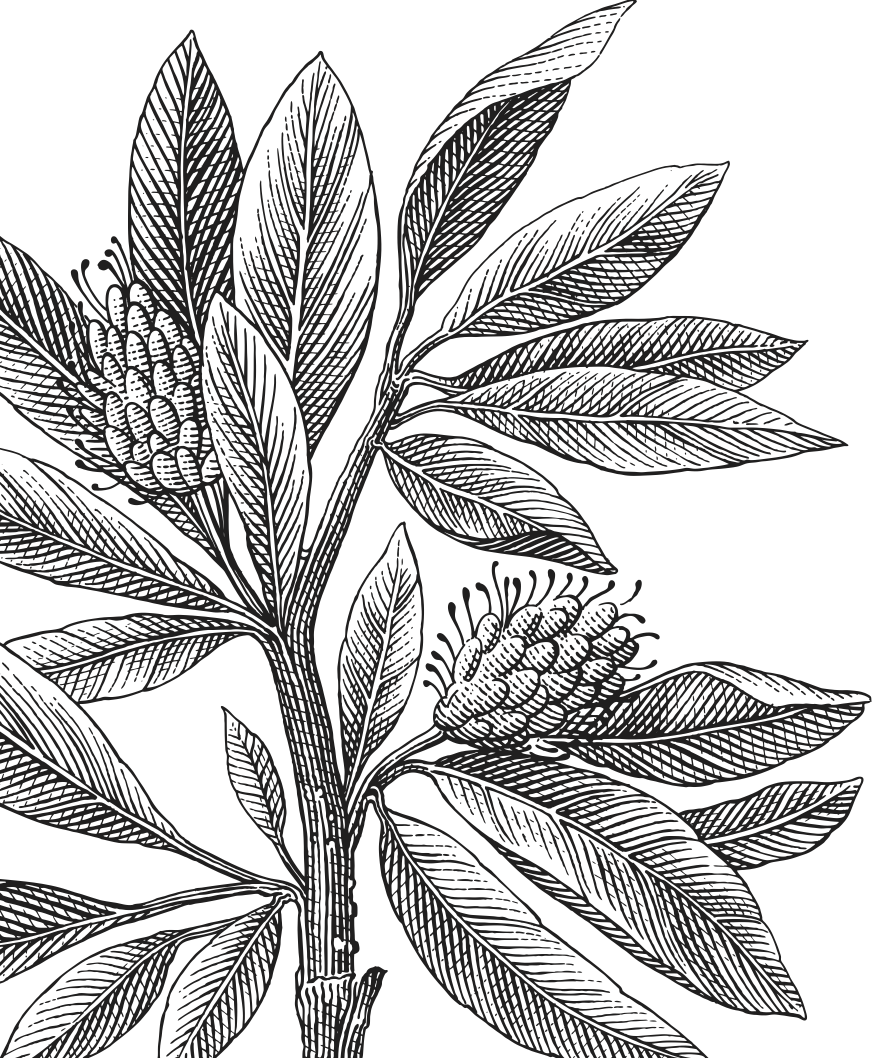
\includegraphics[keepaspectratio,scale=0.3]{lnu_etch.png} % Background picture
    }
}
\newcommand\BackgroundPicLogo{
    \put(30,740){
    
\includegraphics[keepaspectratio,scale=0.10]{logo.png} % Logo in upper left corner
    }
}

\title{	
\vspace{-8cm}
\begin{sidebar}
    \vspace{10cm}
    \normalfont \normalsize
    \Huge \sf Bachelor Thesis \\
    \vspace{-1.3cm}
\end{sidebar}
\vspace{3cm}
\begin{flushleft}
    \huge \bf Optimizing Queueing Performance in Distributed Systems\\
    \it \LARGE - A Queueing Theory Approach with RabbitMQ
\end{flushleft}
\null
\vfill
\begin{textblock}{6}(10,13)
\begin{flushright}
\begin{minipage}{\textwidth}
\begin{flushleft} \normalsize
\emph{Author:} Andreas Lymalm\\
\emph{Supervisor:} Andreas Petersson\\
\emph{Examiner:} Roger Pettersson\\ 
\emph{Semester:} Spring 2025 \\ %
\emph{Subject:} Mathematics (2MA41E) \\ % Subject area
\end{flushleft}
\end{minipage}
\end{flushright}
\end{textblock}
}

\date{}

\begin{document}
\pagenumbering{gobble}
\newgeometry{left=5cm}
\AddToShipoutPicture*{\BackgroundPic}
\AddToShipoutPicture*{\BackgroundPicLogo}
\maketitle
\restoregeometry
\clearpage
%----------------------------------------------------------------------------------------
%	Abstract
%----------------------------------------------------------------------------------------
\selectlanguage{english}
\begin{abstract}

\end{abstract}

\newpage
%----------------------------------------------------------------------------------------
%	Acknowledgements
%----------------------------------------------------------------------------------------

\section*{Acknowledgements}


%----------------------------------------------------------------------------------------
\newpage
\pagenumbering{gobble}
\tableofcontents % Table of contents
\newpage
\pagenumbering{arabic}

%----------------------------------------------------------------------------------------
%
%	Here follows the actual text contents of the report.
%
%----------------------------------------------------------------------------------------

\section{Introduction}

\section{Theoretical Background}

    \subsection{Queueing Theory}
    Queueing theory is the mathematical study of queues, which can be applied, e.g., in systems like computer networks, manufacturing, and service systems. It provides a framework for analyzing how \textit{entities} (such as messages, tasks, or customers) arrive, wait, and are served in a system. 

        \subsubsection{Characteristics}
        The main characteristics of queueing systems include arrival patterns, service patterns, queue disciplines, system capacity, number of servers, and number of service stages \cite{shortle2018}.
        
        \textit{Arrival patterns} defines how entities arrive in the system. For example, in transportation systems it could be a scheduled arrival process, but in many systems a so called \textit{Poisson arrival process} is often used, which models random independent arrivals.

        \textit{Service patterns} defines how entities are processed, with respect to service times, in the system. Some examples are exponential service times for e.g. call centers and deterministic processing times in e.g. manufacturing systems. 

        \textit{Queue disciplines} defines server order rules of the system, such as First-Come-First-Served (FCFS), Last-Come-First-Served (LCFS), and priority queues used in emergency services.

        \textit{System capacity} defines the limits on the number of entities a system can handle. Examples include finite queue lengths in computer buffers and unlimited queue sizes in cloud-based message systems.

        \textit{Number of servers} defines the number of servers in the system. For example, an ATM is a single-server system, while the cashiers in the supermarket are part of a multiple-server system. 

        \textit{Number of service stages} defines the number of steps in the system. A several-step system could be a drive-through in a fast food restaurant, where customers order, pay, and finally receive their food. 

        \subsubsection{Queueing Models}
        To mathematically analyze the performance of a queueing system, there are, with respect to the main characteristics, some common models that are used, and that will be of special interest for this thesis. Specifically, these systems are focusing on the arrival pattern, service pattern, and the number of systems \cite{shortle2018}. 

        The \textit{M/M/1} queue model is a single-server queue system (represented by the \textit{1}), where arrivals follow a Poisson arrival process (represented by the first \textit{M}) and service times are exponentially distributed (represented by the second \textit{M}). 
        
        The \textit{M/M/c} queue model is the same as the former model, but features multiple servers (represented by the \textit{c}).
        
        The \textit{M/G/1} queue model is a single-server system with a Poisson arrival process, like the first model, but which service times follows a general arbitrary distribution (represented by the \textit{G}).
    
    \subsection{Traffic Modeling}
    Traffic modeling builds on queue arrival patterns, focusing on varying demand impacting arrivals. These are the models of interest \cite{ross2022}.

    A \textit{Poisson Arrival Process}, as described in the characteristics chapter, assumes that entities arrive randomly and independently over time and is widely used to model network systems.

\section{Methods}

    \subsection{Mathematical Modeling}
    
    \subsection{Simulation Setup}
    To start with the simulation, we need to first install \textit{Python} (version 3) and the libraries \textit{SimPy} (to simulate queues), \textit{Random} (to generate a random number according to some distribution), and \textit{NumPy} (to analyze any result).

    In Python code, we may now simulate a queueing system by creating an environment (to keep track of waiting times without actually waiting) and a server to service the requests (one entity at a time). In the environment, we can then run an arrival process for a specified amount of simulation time. The final result will be a list of waiting times during the simulation time, which we will start by defining.

    \begin{python}
wait_times = []
env = simpy.Environment()
server = simpy.Resource(env, capacity=1)
env.process(arrival_process(env, server))
env.run(until=SIMULATION_TIME)
    \end{python}

    The arrival process in question should then be set up as an eternal loop of arriving entities, which will not actually be eternal since we will stop after \pythoninline{SIMULATION_TIME}. The arrival loop will consist of two parts; first we should wait a random amount of time according to an exponential distribution with \(\lambda\) \pythoninline{=ARRIVAL_RATE}, being the Poisson arrival process, and secondly, after waiting, we should ask the server to serve the entity. 

    \begin{python}
def arrival_process(env, server):
    request_id = 0
    while True:
        yield env.timeout(random.expovariate(ARRIVAL_RATE)) 
        env.process(serve_request(env, server, request_id))
        request_id += 1
    \end{python}

    The serve request will then serve the request, that will take a random amount of time according to e.g. an exponential distribution with \(\lambda\) \pythoninline{=SERVICE_RATE}, if it's an \(M/M/1\) or \(M/M/c\) system (being determined by the second \(M\)). The waiting time for that request will then be saved in the waiting-times list. 

    \begin{python}
def serve_request(env, server, request_id):
    arrival_time = env.now

    with server.request() as req:
        yield req
        yield env.timeout(random.expovariate(SERVICE_RATE))
    
    wait_time = env.now - arrival_time
    wait_times.append(wait_time)
    \end{python}

    Running this code, which is set up for \(M/M/1\), we can now compare the average waiting time in an ideal simulation environment with the exact mathematical value, for different values for \pythoninline{ARRIVAL_RATE}, \pythoninline{SERVICE_RATE}, and \pythoninline{SIMULATION_TIME}.
    
    \subsection{Experimental Setup}
    So, in contrast to the previous section where we set up an ideal simulation, we will in this section set up a simulation with as much disturbance as possible, in various ways and combinations. 
    
    To start, we should install \textit{RabbitMQ} and the libraries \textit{pika} (to communicate with \textit{RabbitMQ}) and \textit{time} (to track time) for \textit{Python}. Then, we start RabbitMQ by running e.g. 
    \begin{lstlisting}[style=DOS]
    rabbitmq-server
    \end{lstlisting}
    for \textit{Windows}. 

    As for the code setup, we can set up the communication with RabbitMQ by specifiying where it is running on the computer, which should now be localhost, and then setting up a connection and a queue. 

    \begin{python}
parameters = pika.ConnectionParameters('localhost')
connection = pika.BlockingConnection(parameters)
channel = connection.channel()
channel.queue_declare(queue='mm1_queue')
    \end{python}

    Now, we want to create a producer and a consumer. The producer will generate requests (the entities) that will be sent to RabbitMQ via the shared channel, which will queue the request and later send it to the consumer (the server) for processing. The producer will send along the time at which the request were made, which will be useful for the consumer. would send request like follows.

    \begin{python}
def send_request():
    message = str(time.time())
    channel.basic_publish(exchange='', routing_key='mm1_queue', body=message)
    time.sleep(random.expovariate(ARRIVAL_RATE))
    \end{python}

    The consumer will be on the other end of the channel and continuously listen for any incoming requests. 

    \begin{python}
channel.basic_consume(queue=QUEUE_NAME, on_message_callback=serve_request)
channel.start_consuming()
    \end{python}

    When a request is received, it will run the \pythoninline{serve_request} function. There, similar functionality as in the previous chapter's \pythoninline{serve_request} function is executed. A key difference here is that the consumer needs to tell RabbitMQ that the request has been processed, or it will be stuck in the queue. 

    \begin{python}
def serve_request(ch, method, properties, body):
    arrival_time = float(body.decode()) # Producer data
    service_time = random.expovariate(SERVICE_RATE)
    time.sleep(service_time)
    
    wait_time = time.time() - arrival_time
    wait_times.append(wait_time)
    
    ch.basic_ack(delivery_tag=method.delivery_tag)
    \end{python}

\section{Results}

    \subsection{Simulation Results}

    \subsection{Experimental Results}

    \subsection{Comparison}

\section{Discussion}

%----------------------------------------------------------------------------------------
%	List of References
%-----------------------------------------------------------------------------------------


\hypersetup{urlcolor=black}
\bibliographystyle{IEEEtran}
\bibliography{references}
\newpage

%----------------------------------------------------------------------------------------
%	Appendices
%-----------------------------------------------------------------------------------------

\appendix

\section{Appendix 1}


\end{document}
